
\chapter{Wyniki dla pozostałych maszyn wirtualnych}

\begin{table}[p]
	\begin{center}        
 		\begin{tabular}{l r r r r } \toprule
 & \emph{bpr} & \emph{divsufsort} & \emph{qsufsort} & \emph{skew}\\ \midrule
\texttt{abac} & 1.04 & 0.01 & \textbf{0.01} & 0.05\\
\texttt{abba} & 4.23 & \textbf{2.19} & 2.26 & 11.23\\
\texttt{book1x20} & \textbf{3.14} & 3.29 & 3.40 & 22.52\\
\texttt{fib\_s14930352} & 10.05 & 4.94 & \textbf{3.32} & 14.09\\
\texttt{fss10} & 5.36 & 3.88 & \textbf{2.69} & 12.34\\
\texttt{fss9} & 1.05 & 0.63 & \textbf{0.58} & 1.89\\
\texttt{houston} & 2.63 & \textbf{0.24} & 0.44 & 0.96\\
\texttt{paper5x80} & 0.18 & 0.15 & \textbf{0.08} & 0.42\\
\texttt{test1} & 2.26 & 0.41 & \textbf{0.20} & 1.91\\
\texttt{test2} & 0.71 & 0.34 & \textbf{0.20} & 1.91\\
\texttt{test3} & 74.40 & 0.42 & \textbf{0.37} & 0.91\\
 \midrule
Total & 105.05 & 16.49 & \textbf{13.55} & 68.24\\
 \bottomrule
\end{tabular}

    \end{center}                         
	\caption{Czas działania algorytmów na plikach z korpusu \texttt{The Gauntlet} dla maszyny wirtualnej \texttt{ibm}.}%
    \label{tab:ibm-gauntlet}
\end{table}

\begin{figure}[p]
   \begin{center}
        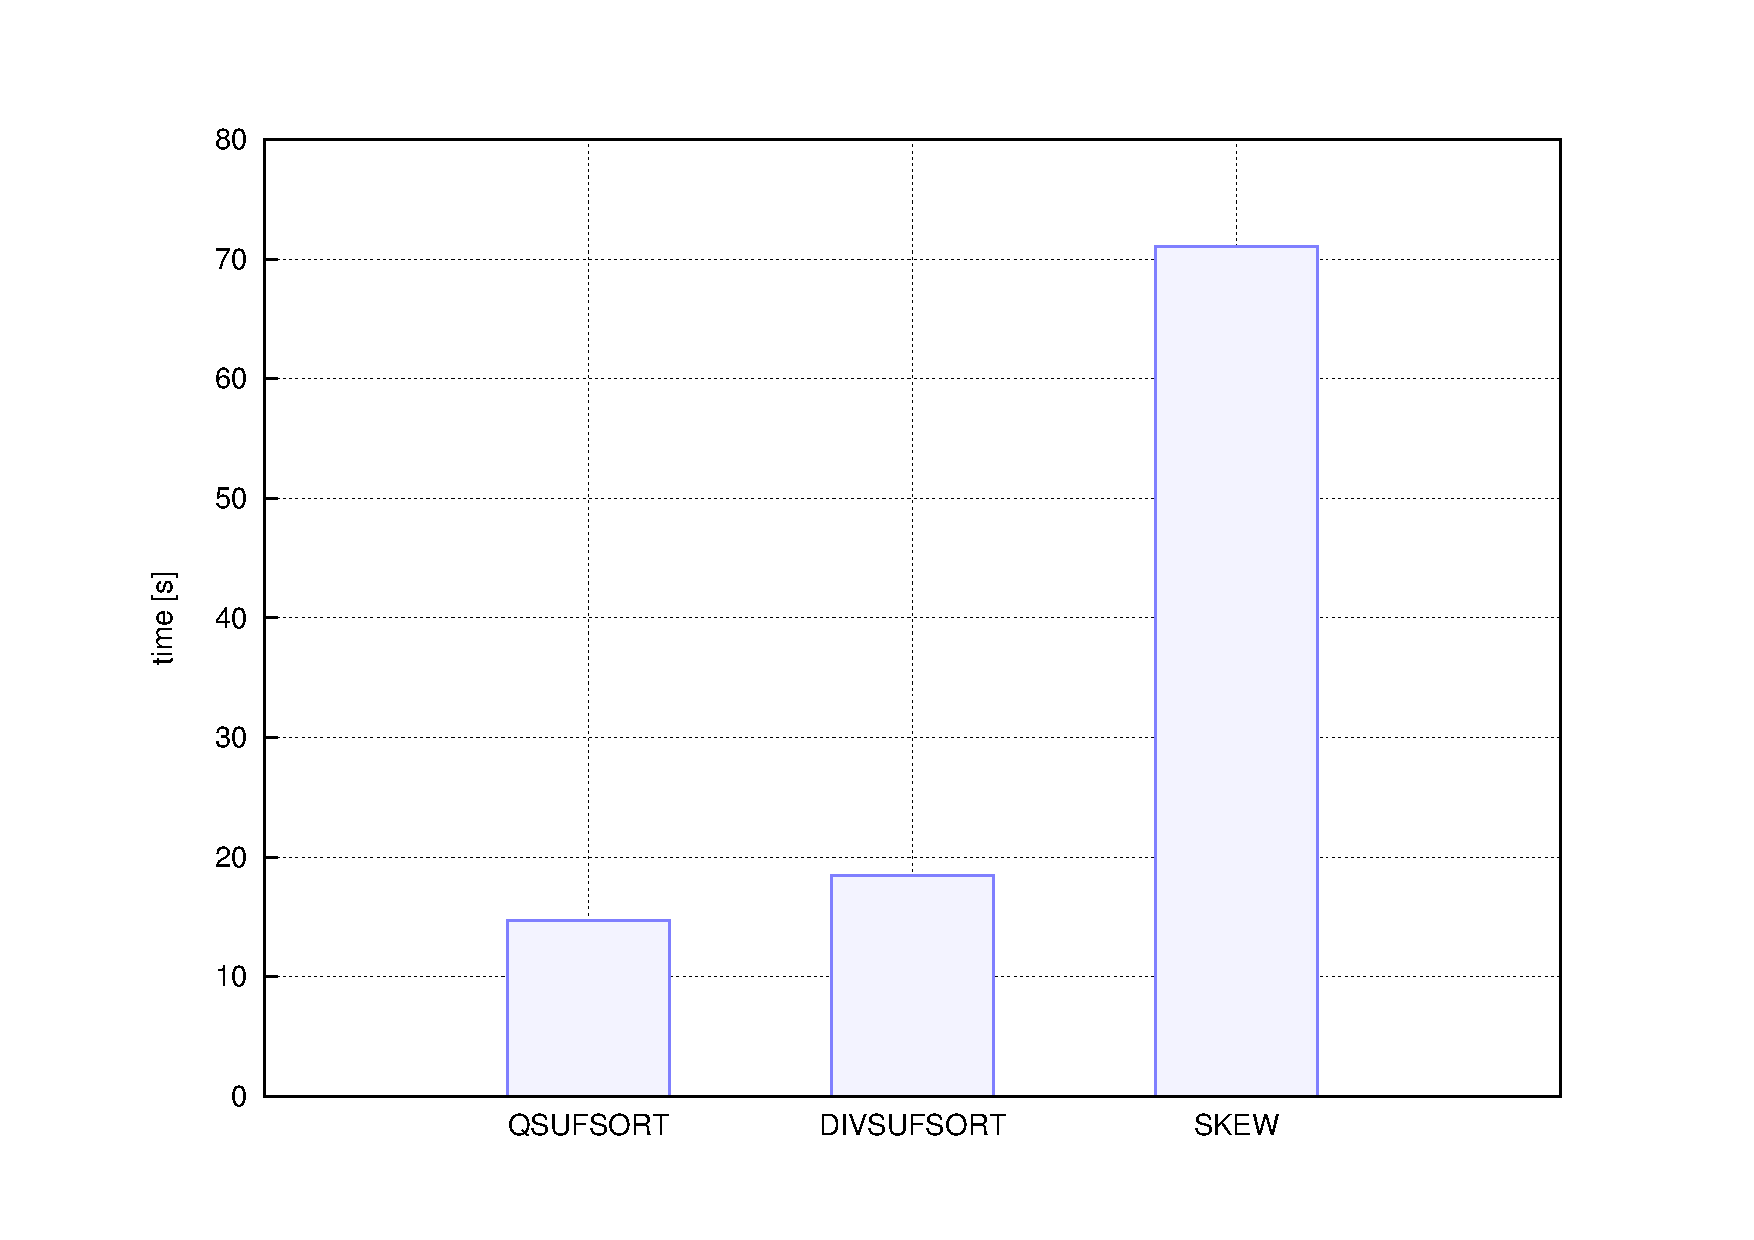
\includegraphics[width=\linewidth]{figures/results/ibm-gauntlet.pdf}
    \end{center}        
    \caption{Sumaryczny czas działania algorytmów na plikach z korpusu \texttt{The Gauntlet} dla maszyny wirtualnej \texttt{ibm}.}%
    \label{rys:ibm-gauntlet}
\end{figure}


\begin{table}[p]
	\begin{center}        
 		\begin{tabular}{l r r r r } \toprule
 & \emph{bpr} & \emph{divsufsort} & \emph{qsufsort} & \emph{skew}\\ \midrule
\texttt{chr22.dna} & \textbf{6.22} & 7.62 & 7.29 & 59.27\\
\texttt{etext99} & 25.38 & 59.93 & \textbf{25.21} & ---\\
\texttt{gcc-3.0.tar} & 19.56 & 37.32 & \textbf{14.07} & ---\\
\texttt{howto} & 7.43 & 8.05 & \textbf{7.20} & 78.05\\
\texttt{jdk13c} & 14.50 & 24.81 & \textbf{11.44} & ---\\
\texttt{linux-2.4.5.tar} & 23.68 & 57.76 & \textbf{19.53} & ---\\
\texttt{rctail96} & 28.61 & 56.08 & \textbf{23.49} & ---\\
\texttt{rfc} & 26.42 & 53.69 & \textbf{23.39} & ---\\
\texttt{sprot34.dat} & 26.51 & 65.53 & \textbf{21.90} & ---\\
\texttt{w3c2} & 22.53 & 45.49 & \textbf{16.43} & ---\\
 \midrule
Total & 200.84 & 416.30 & \textbf{169.95} & \\
 \bottomrule
\end{tabular}
 
    \end{center}                         
	\caption{Czas działania algorytmów na plikach z korpusu Giovanniego Manziniego dla maszyny wirtualnej \texttt{ibm}.}%
    \label{tab:ibm-manzini}
\end{table}

\begin{figure}[p]
       \begin{center}
            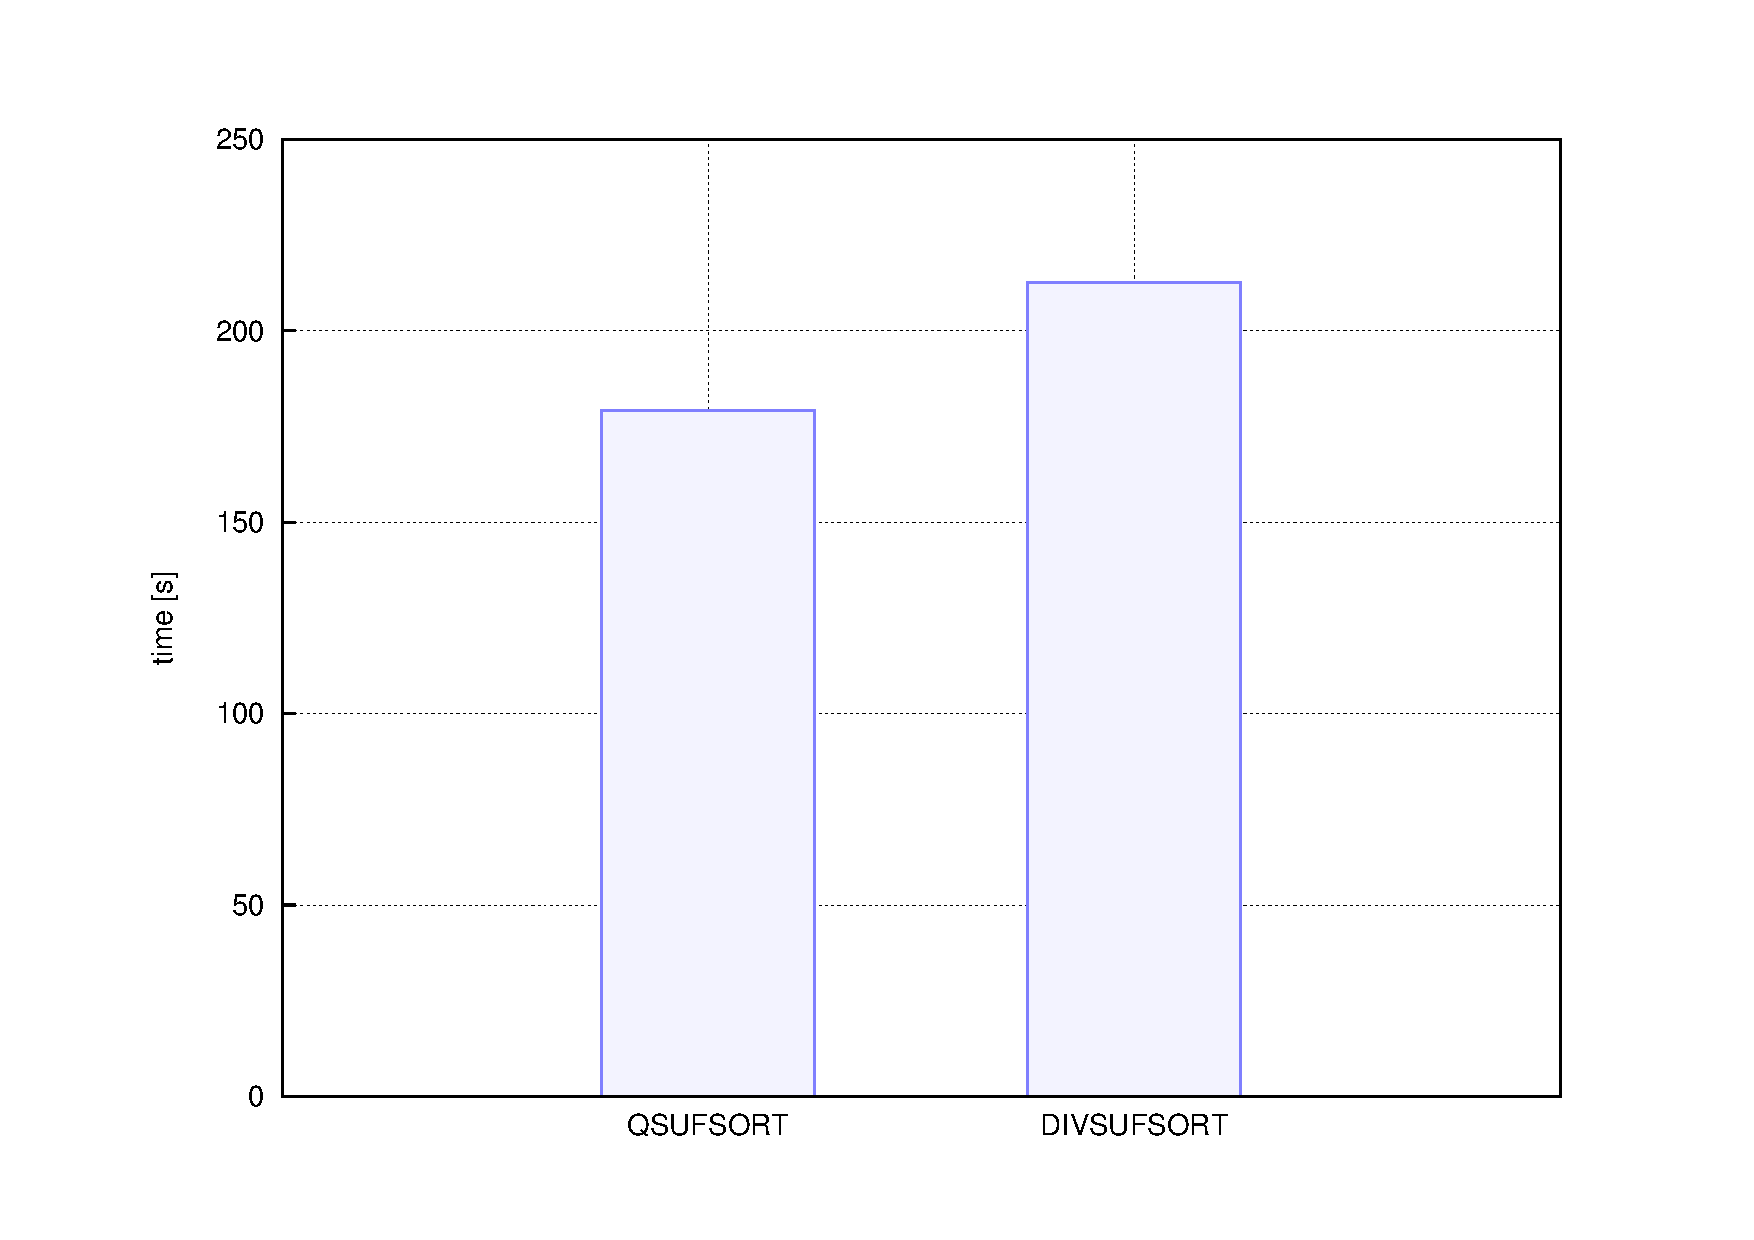
\includegraphics[width=\linewidth]{figures/results/ibm-manzini.pdf}
        \end{center}        
	    \caption{Sumaryczny czas działania algorytmów na plikach z korpusu Giovanniego Manziniego dla maszyny wirtualnej \texttt{ibm}.}%
    \label{rys:ibm-manzini}
\end{figure}
 

\begin{table}[p]
	\begin{center}        
 		\begin{tabular}{l r r r r } \toprule
 & \emph{bpr} & \emph{divsufsort} & \emph{qsufsort} & \emph{skew}\\ \midrule
\texttt{abac} & 1.04 & 0.01 & \textbf{0.01} & 0.05\\
\texttt{abba} & 4.23 & \textbf{2.19} & 2.26 & 11.23\\
\texttt{book1x20} & \textbf{3.14} & 3.29 & 3.40 & 22.52\\
\texttt{fib\_s14930352} & 10.05 & 4.94 & \textbf{3.32} & 14.09\\
\texttt{fss10} & 5.36 & 3.88 & \textbf{2.69} & 12.34\\
\texttt{fss9} & 1.05 & 0.63 & \textbf{0.58} & 1.89\\
\texttt{houston} & 2.63 & \textbf{0.24} & 0.44 & 0.96\\
\texttt{paper5x80} & 0.18 & 0.15 & \textbf{0.08} & 0.42\\
\texttt{test1} & 2.26 & 0.41 & \textbf{0.20} & 1.91\\
\texttt{test2} & 0.71 & 0.34 & \textbf{0.20} & 1.91\\
\texttt{test3} & 74.40 & 0.42 & \textbf{0.37} & 0.91\\
 \midrule
Total & 105.05 & 16.49 & \textbf{13.55} & 68.24\\
 \bottomrule
\end{tabular}

    \end{center}                         
	\caption{Czas działania algorytmów na plikach z korpusu \texttt{The Gauntlet} dla maszyny wirtualnej \texttt{jrockit}.}%
    \label{tab:jrockit-gauntlet}
\end{table}

\begin{figure}[p]
       \begin{center}
            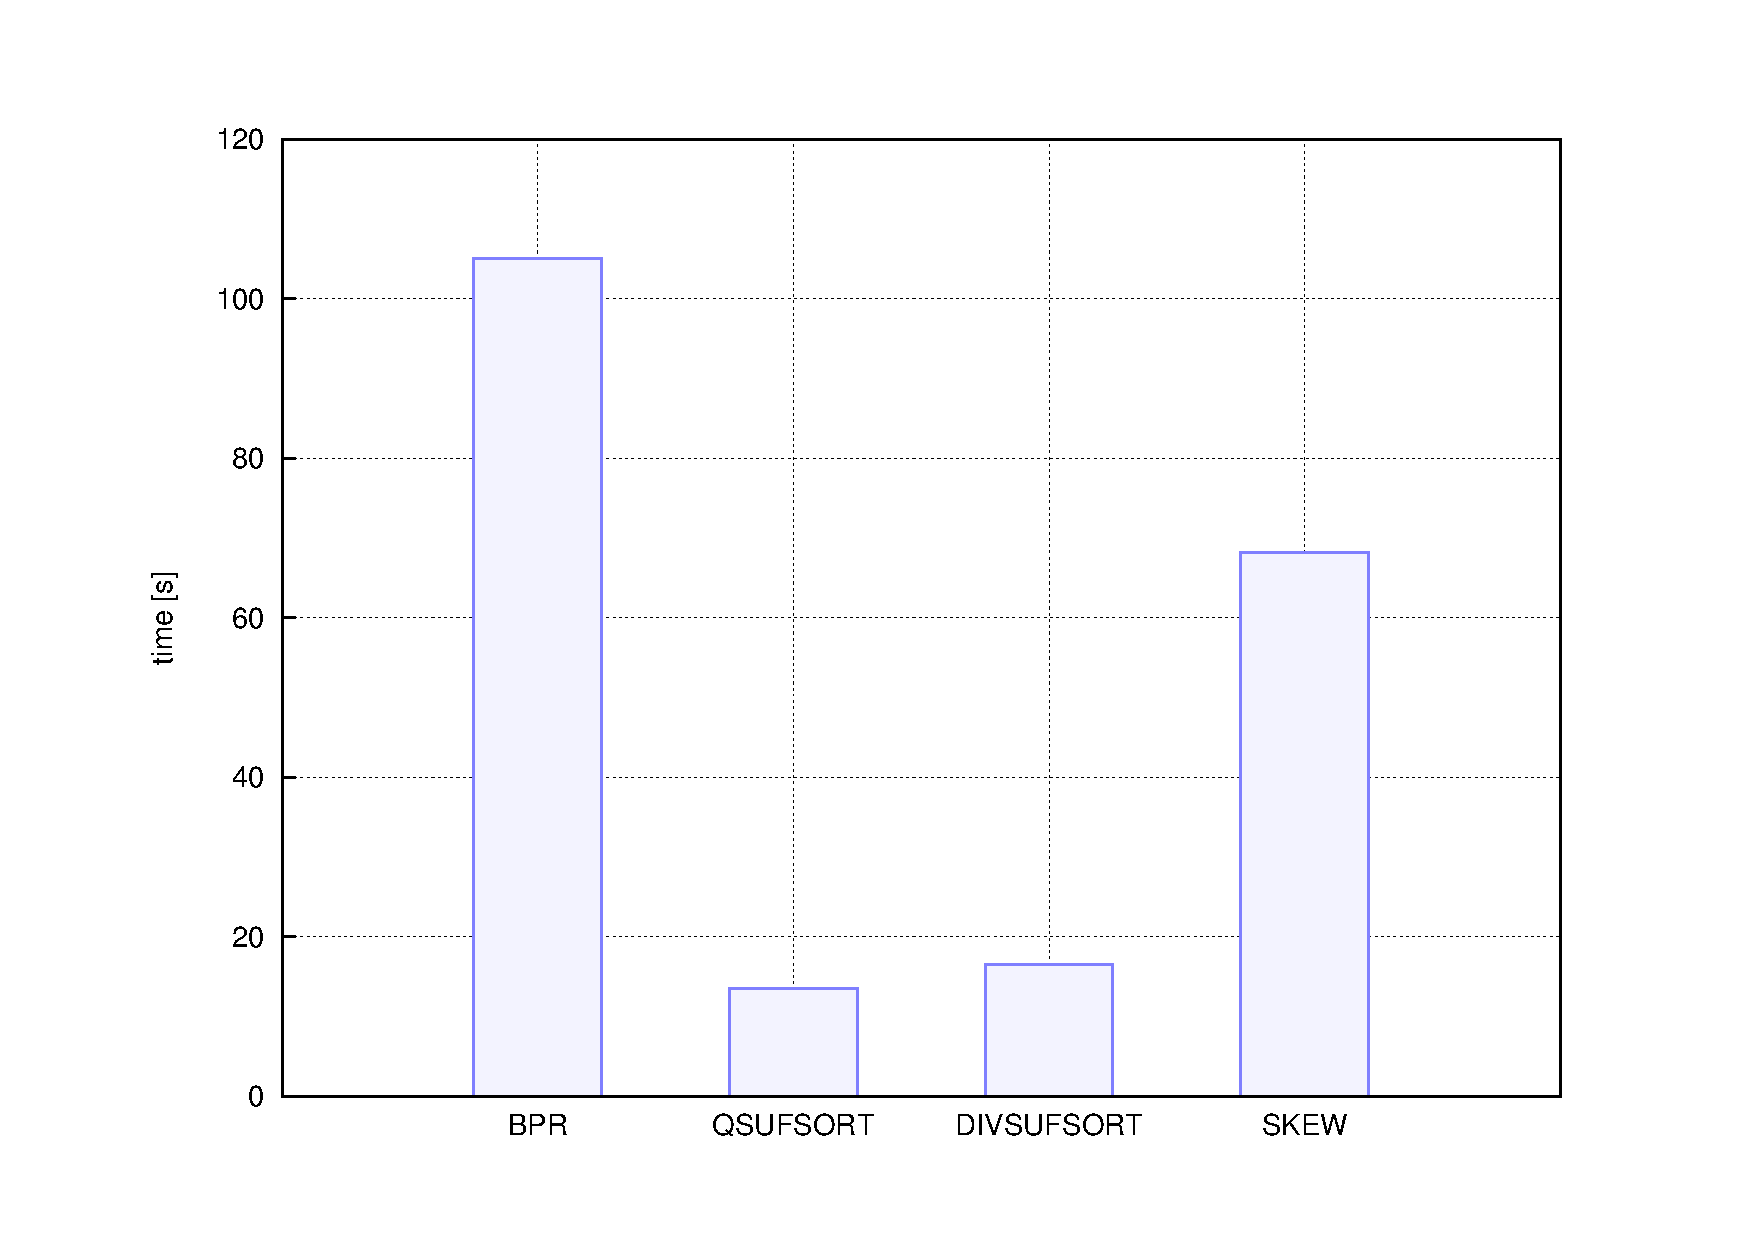
\includegraphics[width=\linewidth]{figures/results/jrockit-gauntlet.pdf}
        \end{center}        
	    \caption{Sumaryczny czas działania algorytmów na plikach z korpusu \texttt{The Gauntlet} dla maszyny wirtualnej \texttt{jrockit}.}%
    \label{rys:jrockit-gauntlet}
\end{figure} 


\begin{table}[p]
	\begin{center}        
 		\begin{tabular}{l r r r r } \toprule
 & \emph{bpr} & \emph{divsufsort} & \emph{qsufsort} & \emph{skew}\\ \midrule
\texttt{chr22.dna} & \textbf{6.22} & 7.62 & 7.29 & 59.27\\
\texttt{etext99} & 25.38 & 59.93 & \textbf{25.21} & ---\\
\texttt{gcc-3.0.tar} & 19.56 & 37.32 & \textbf{14.07} & ---\\
\texttt{howto} & 7.43 & 8.05 & \textbf{7.20} & 78.05\\
\texttt{jdk13c} & 14.50 & 24.81 & \textbf{11.44} & ---\\
\texttt{linux-2.4.5.tar} & 23.68 & 57.76 & \textbf{19.53} & ---\\
\texttt{rctail96} & 28.61 & 56.08 & \textbf{23.49} & ---\\
\texttt{rfc} & 26.42 & 53.69 & \textbf{23.39} & ---\\
\texttt{sprot34.dat} & 26.51 & 65.53 & \textbf{21.90} & ---\\
\texttt{w3c2} & 22.53 & 45.49 & \textbf{16.43} & ---\\
 \midrule
Total & 200.84 & 416.30 & \textbf{169.95} & \\
 \bottomrule
\end{tabular}
 
    \end{center}                         
\caption{Czas działania algorytmów na plikach z korpusu Giovanniego Manziniego dla maszyny wirtualnej \texttt{jrockit}.}%
    \label{tab:jrockit-manzini}
\end{table}

\begin{figure}[p]
       \begin{center}
            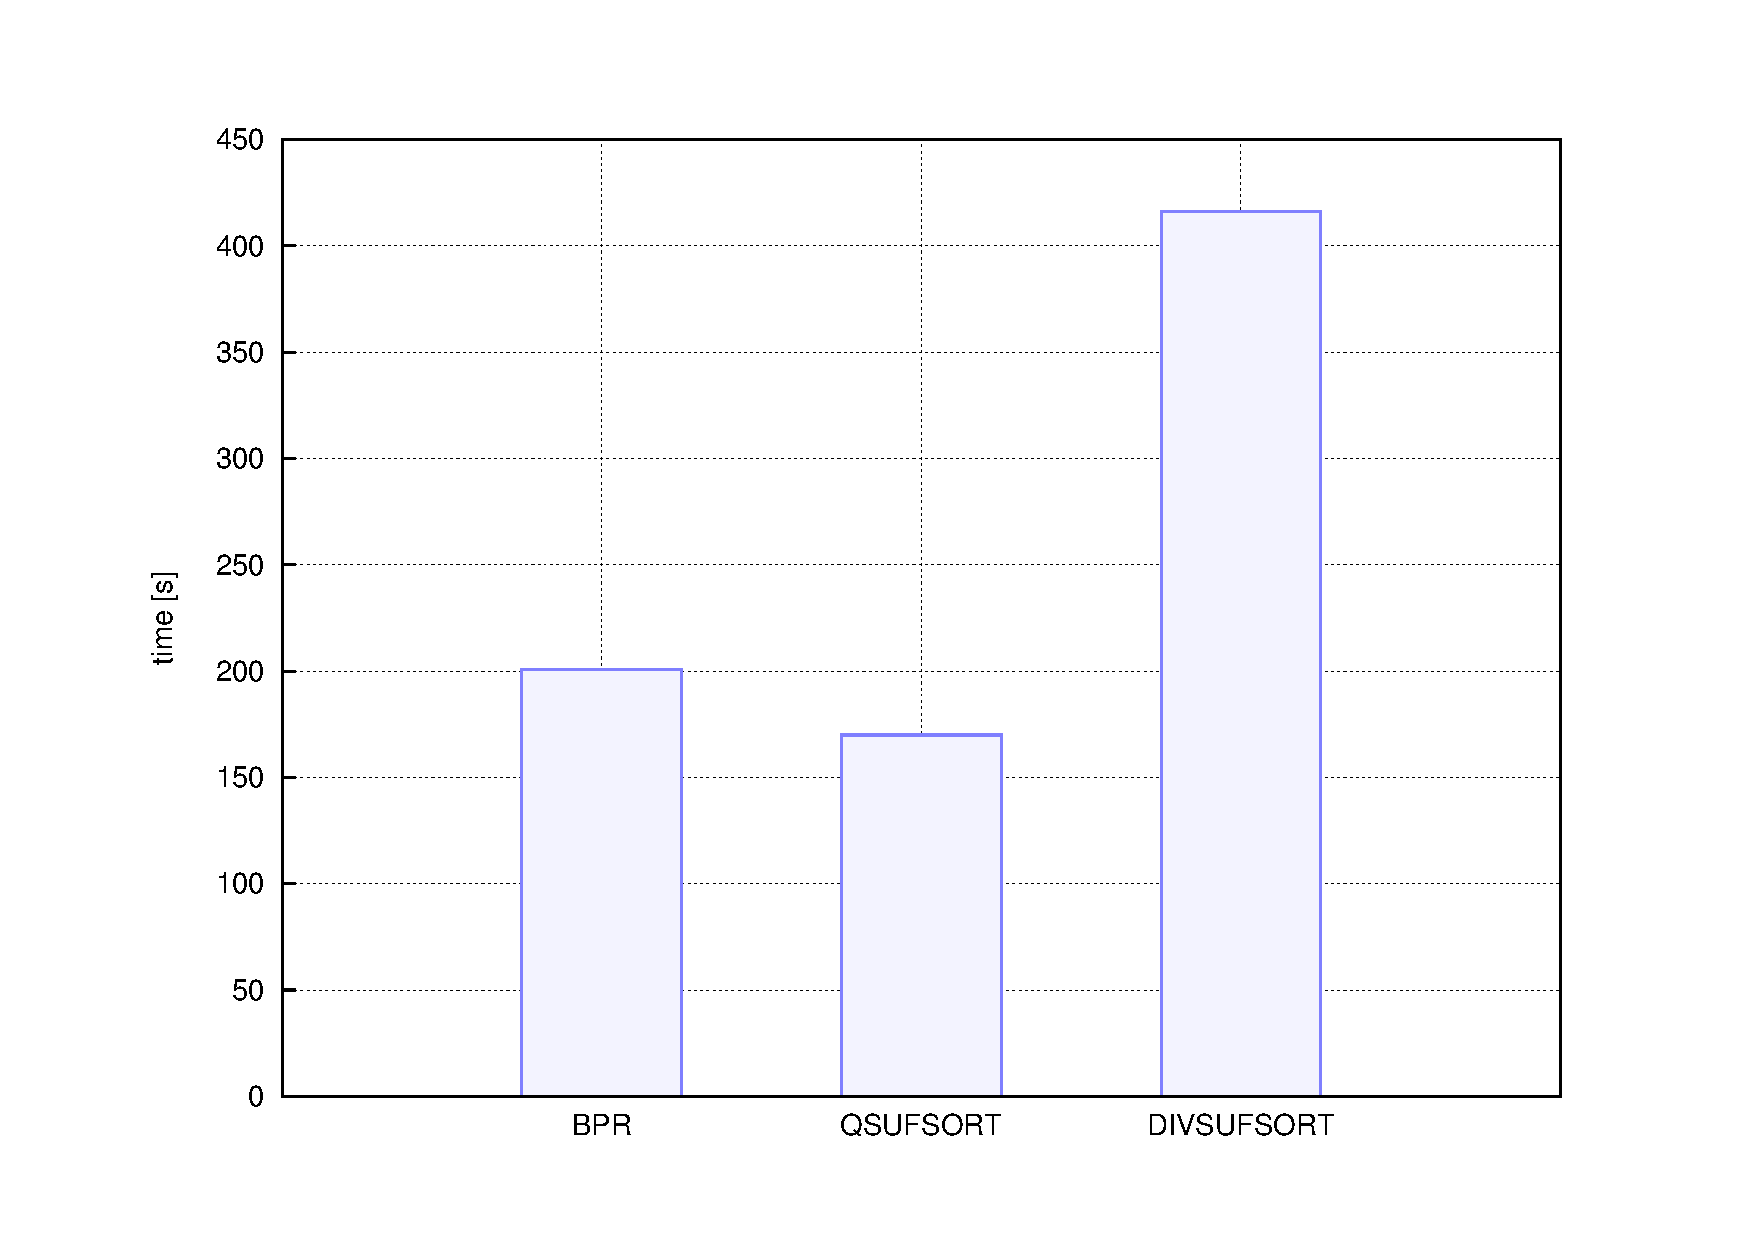
\includegraphics[width=\linewidth]{figures/results/jrockit-manzini.pdf}
        \end{center}        
	    \caption{Sumaryczny czas działania algorytmów na plikach z korpusu Giovanniego Manziniego dla maszyny wirtualnej \texttt{jrockit}.}%
    \label{rys:jrockit-manzini}
\end{figure} 


\begin{table}[p]
	\begin{center}        
 		\begin{tabular}{l r r r r } \toprule
 & \emph{bpr} & \emph{divsufsort} & \emph{qsufsort} & \emph{skew}\\ \midrule
\texttt{abac} & 1.04 & 0.01 & \textbf{0.01} & 0.05\\
\texttt{abba} & 4.23 & \textbf{2.19} & 2.26 & 11.23\\
\texttt{book1x20} & \textbf{3.14} & 3.29 & 3.40 & 22.52\\
\texttt{fib\_s14930352} & 10.05 & 4.94 & \textbf{3.32} & 14.09\\
\texttt{fss10} & 5.36 & 3.88 & \textbf{2.69} & 12.34\\
\texttt{fss9} & 1.05 & 0.63 & \textbf{0.58} & 1.89\\
\texttt{houston} & 2.63 & \textbf{0.24} & 0.44 & 0.96\\
\texttt{paper5x80} & 0.18 & 0.15 & \textbf{0.08} & 0.42\\
\texttt{test1} & 2.26 & 0.41 & \textbf{0.20} & 1.91\\
\texttt{test2} & 0.71 & 0.34 & \textbf{0.20} & 1.91\\
\texttt{test3} & 74.40 & 0.42 & \textbf{0.37} & 0.91\\
 \midrule
Total & 105.05 & 16.49 & \textbf{13.55} & 68.24\\
 \bottomrule
\end{tabular}

    \end{center}                         
	\caption{Czas działania algorytmów na plikach z korpusu \texttt{The Gauntlet} dla maszyny wirtualnej \texttt{harmony}.}%
    \label{tab:harmony-gauntlet}
\end{table}

\begin{figure}[p]
       \begin{center}
            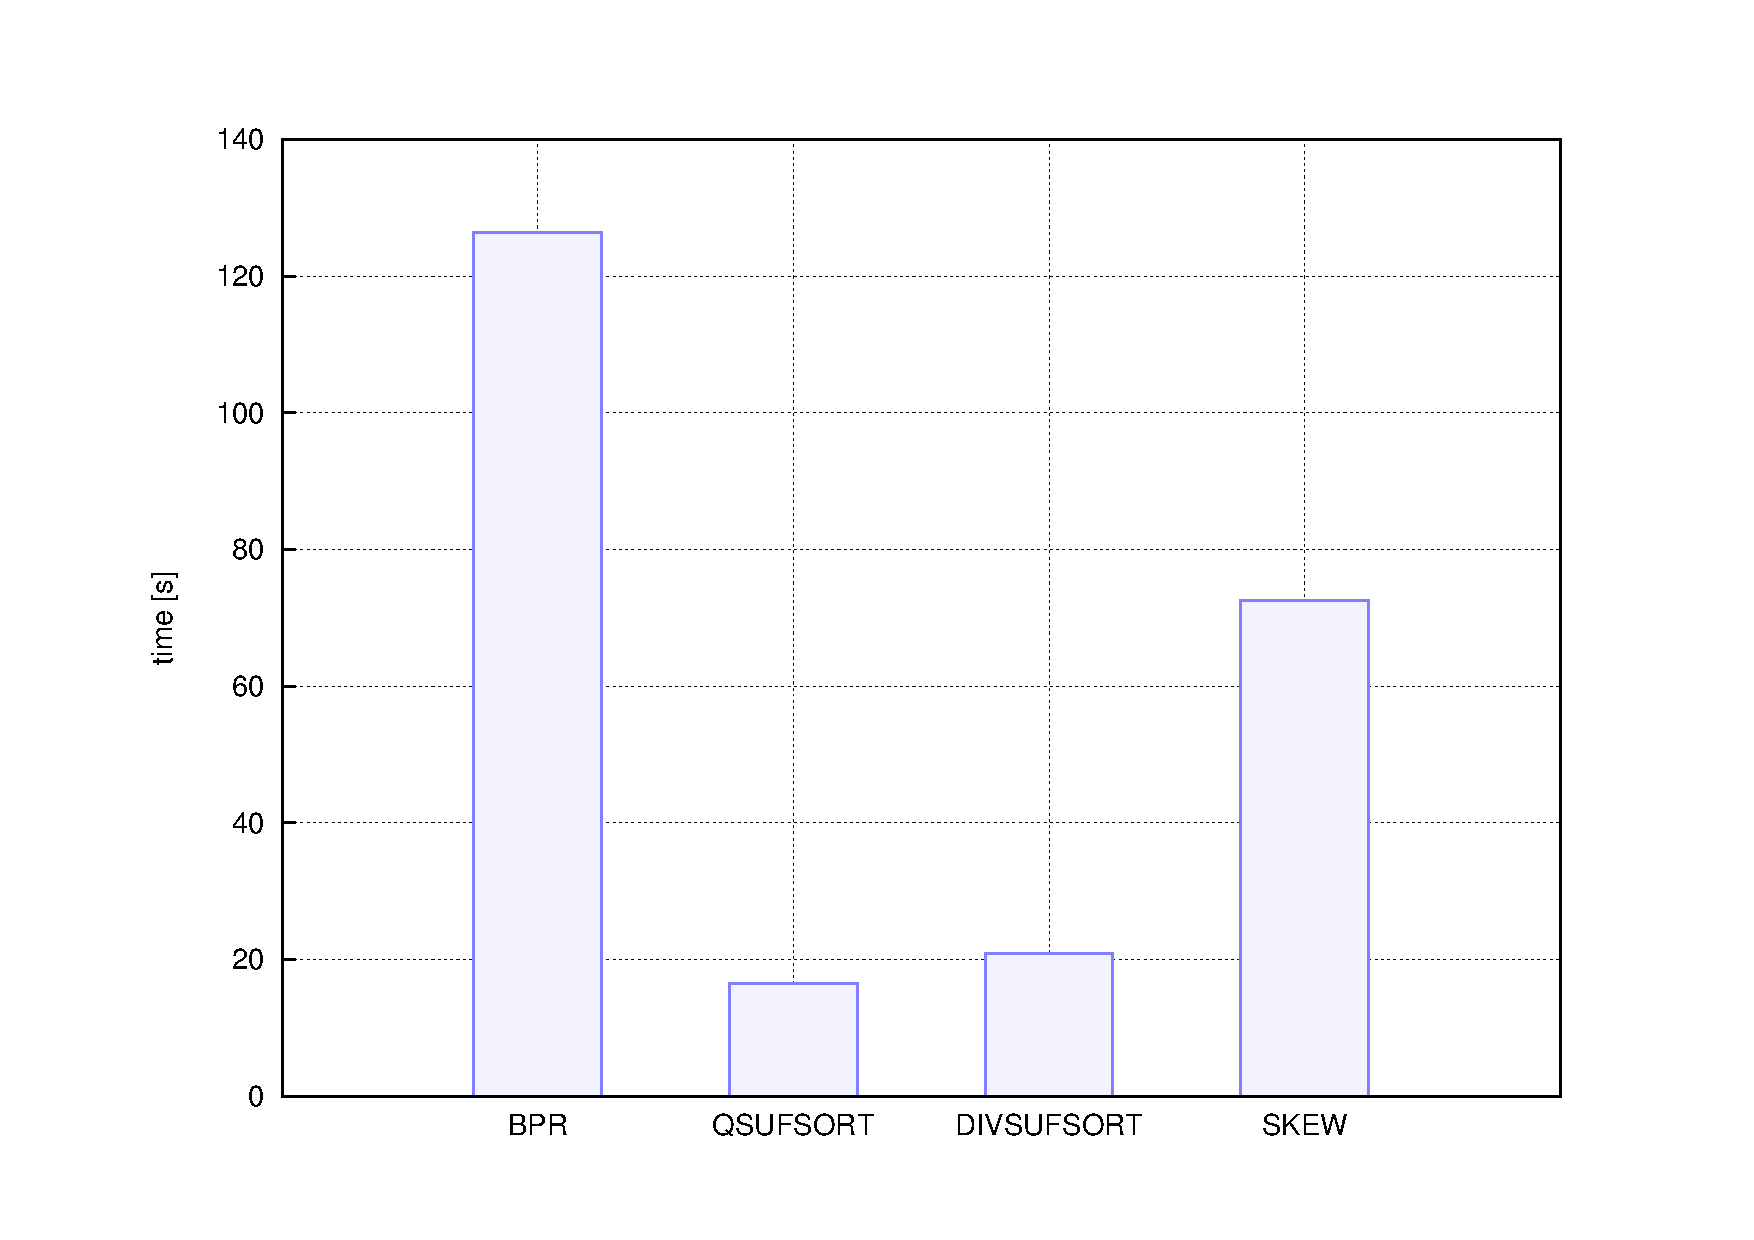
\includegraphics[width=\linewidth]{figures/results/harmony-gauntlet.pdf}
        \end{center}        
	    \caption{Sumaryczny czas działania algorytmów na plikach z korpusu \texttt{The Gauntlet} dla maszyny wirtualnej \texttt{harmony}.}%
    \label{rys:harmony-gauntlet}
\end{figure} 


\begin{table}[p]
	\begin{center}        
 		\begin{tabular}{l r r r r } \toprule
 & \emph{bpr} & \emph{divsufsort} & \emph{qsufsort} & \emph{skew}\\ \midrule
\texttt{chr22.dna} & \textbf{6.22} & 7.62 & 7.29 & 59.27\\
\texttt{etext99} & 25.38 & 59.93 & \textbf{25.21} & ---\\
\texttt{gcc-3.0.tar} & 19.56 & 37.32 & \textbf{14.07} & ---\\
\texttt{howto} & 7.43 & 8.05 & \textbf{7.20} & 78.05\\
\texttt{jdk13c} & 14.50 & 24.81 & \textbf{11.44} & ---\\
\texttt{linux-2.4.5.tar} & 23.68 & 57.76 & \textbf{19.53} & ---\\
\texttt{rctail96} & 28.61 & 56.08 & \textbf{23.49} & ---\\
\texttt{rfc} & 26.42 & 53.69 & \textbf{23.39} & ---\\
\texttt{sprot34.dat} & 26.51 & 65.53 & \textbf{21.90} & ---\\
\texttt{w3c2} & 22.53 & 45.49 & \textbf{16.43} & ---\\
 \midrule
Total & 200.84 & 416.30 & \textbf{169.95} & \\
 \bottomrule
\end{tabular}
 
    \end{center}                         
	\caption{Czas działania algorytmów na plikach z korpusu Giovanniego Manziniego dla maszyny wirtualnej \texttt{harmony}.}%
    \label{tab:harmony-manzini}
\end{table}

\begin{figure}[p]
       \begin{center}
            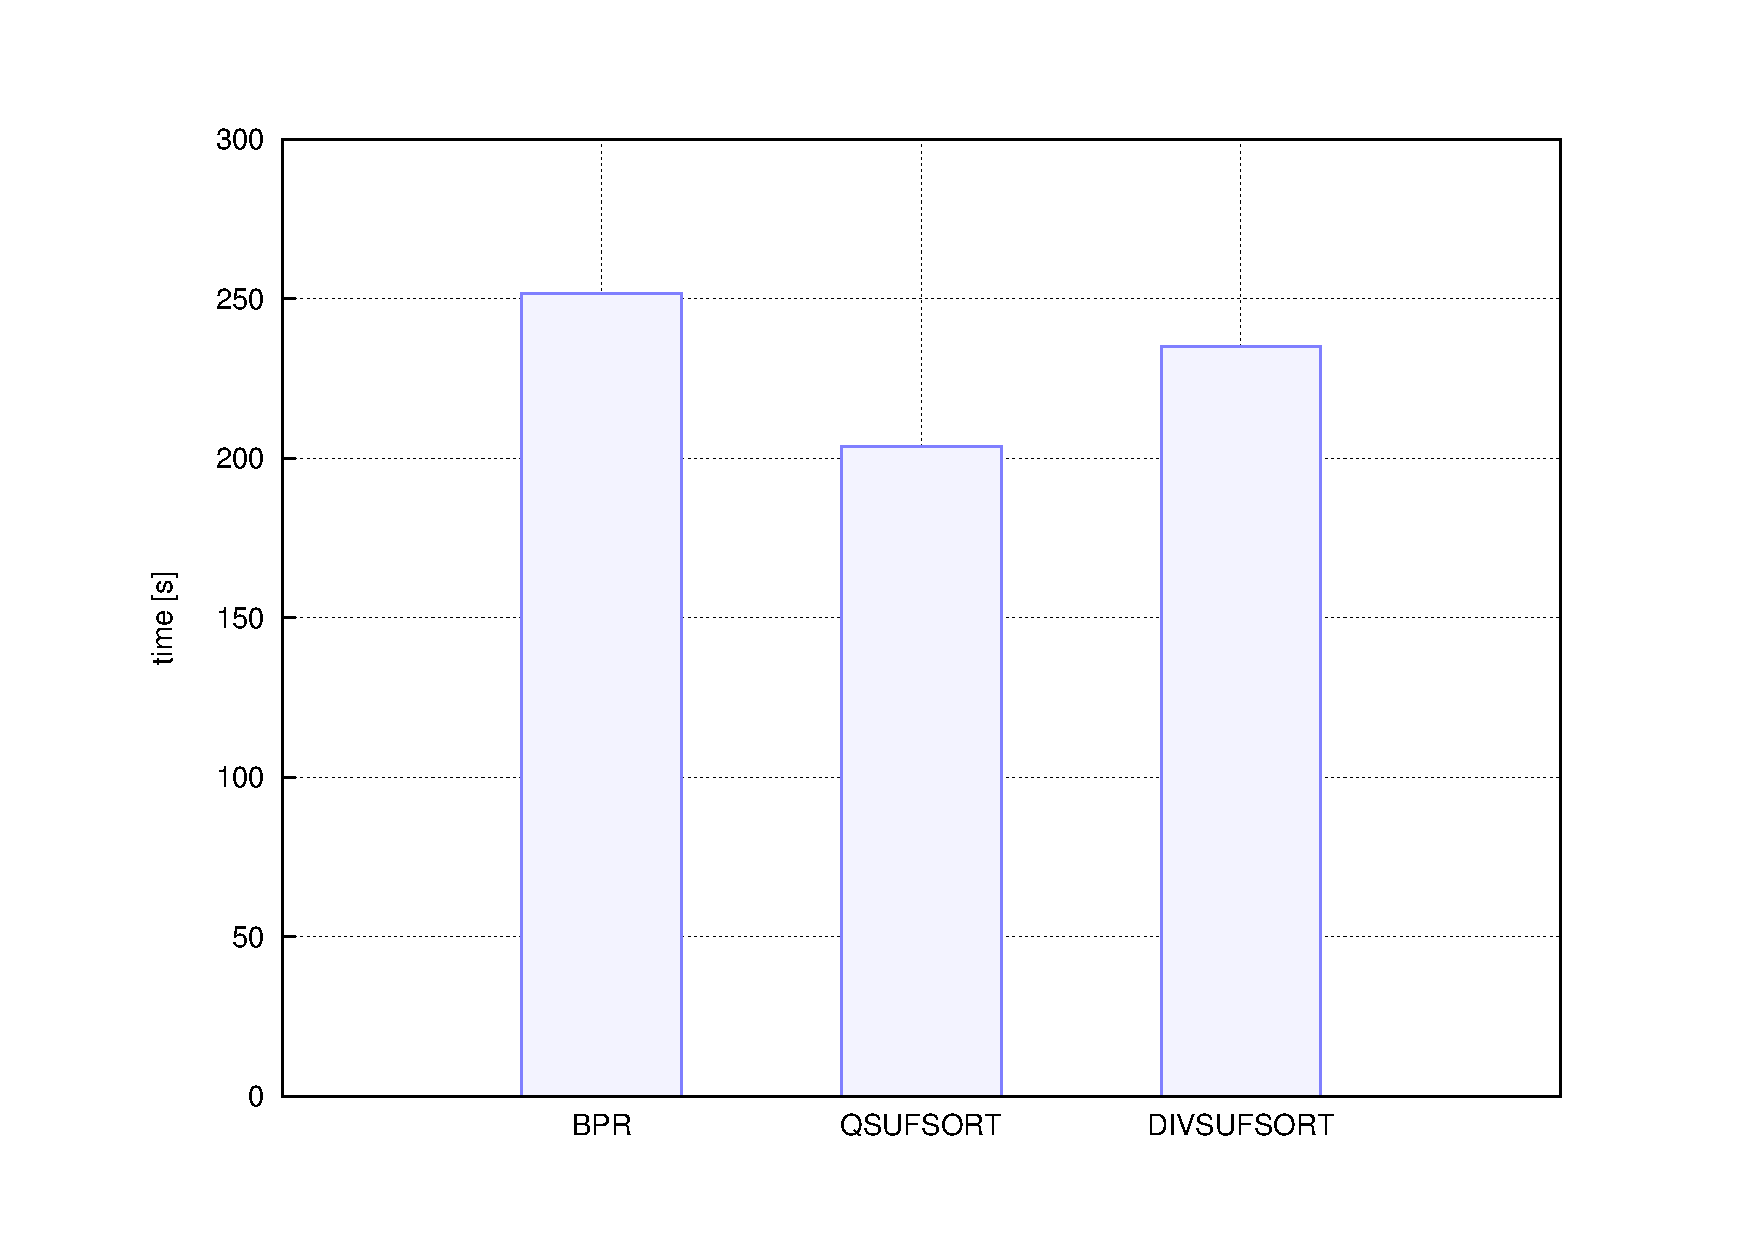
\includegraphics[width=\linewidth]{figures/results/harmony-manzini.pdf}
        \end{center}        
	    \caption{Sumaryczny czas działania algorytmów na plikach z korpusu Giovanniego Manziniego dla maszyny wirtualnej \texttt{harmony}.}%
    \label{rys:harmony-manzini}
\end{figure}
 